%各自の環境に応じて修正
%\documentclass[a4paper,11pt]{jarticle}
\documentclass{ltjsarticle}

\usepackage{enumitem}
\usepackage{appendix}
\usepackage{float}
\usepackage{bm}
\usepackage[dvipdfmx]{graphicx}
\usepackage[dvipdfmx]{color}
\usepackage{tikz}
\usepackage[T1]{fontenc}
\usepackage[utf8]{inputenc}
\usepackage{lmodern}
\usepackage[american]{babel}
\usepackage{subcaption}
\usepackage{tabularx}
\usepackage{graphics}
\usepackage{physics}
\usepackage{mathtools}
\usepackage{amssymb,amsmath,amsfonts,eurosym,geometry,graphicx,caption,color,setspace,comment,footmisc,caption,pdflscape,array,hyperref}
\usepackage{booktabs}
\usepackage{siunitx}
\newcolumntype{d}{S[
    input-open-uncertainty=,
    input-close-uncertainty=,
    parse-numbers = false,
    table-align-text-pre=false,
    table-align-text-post=false
]}
\usepackage{listings} 
\usepackage{xcolor}
\lstdefinestyle{matlab}{
  language=Matlab,
  basicstyle=\ttfamily\footnotesize,
  keywordstyle=\color{blue},
  stringstyle=\color{red},
  commentstyle=\color{green!60!black},
  numbers=left,
  numberstyle=\tiny\color{gray},
  stepnumber=1,
  frame=single,
  breaklines=true,
  showstringspaces=false
}

 
\usepackage{titlesec}
\titleformat*{\section}{\Large\rmfamily}
\titleformat*{\subsection}{\large\rmfamily}
\titleformat*{\subsubsection}{\rmfamily}
 

%テキストの表示領域の調節
\setlength{\textwidth}{\paperwidth}
\addtolength{\textwidth}{-40truemm}
\setlength{\textheight}{\paperheight}
\addtolength{\textheight}{-45truemm}

%余白の調節
\setlength{\topmargin}{-10.4truemm}
\setlength{\evensidemargin}{-5.4truemm}
\setlength{\oddsidemargin}{-5.4truemm}
\setlength{\headheight}{17pt}
\setlength{\headsep}{10mm}
\addtolength{\headsep}{-17pt}
\setlength{\footskip}{5mm}

% \renewcommand{\thesection}{\Alph{section}}
% \renewcommand{\thesubsection}{\alph{subsection}}


\title{Macroeconomics $\mathrm{II}$ Homework 3}
\date{\today}
\author{Graduate School of Economics, The University of Tokyo\\[4mm]29--246029 Rin NITTA\\ 29-246033 Rei HANARI \\ 29--246004 Kosuke IGARASHI}

\begin{document}
\maketitle
\section*{Q1}
\subsection*{(a)}


The recursive formulation of a standard neoclassical growth
model studied in class in Lecture 3 is
\begin{align*}
    v(k)=\max_{0\leq k'\leq f(k)} \qty{U(f(k)-k')+\beta v(k')}.
\end{align*}


Define metricx space $(B(X),d)$, the space of bounded functions on $X=[0,\infty)$ with the sup-norm $d$, and difine operator $T$ as 
\begin{align*}
    Tv(k)=\max_{0\leq k'\leq f(k)} \qty{U(f(k)-k')+\beta v(k')}.
\end{align*}

Then, by showing $T$ satisfies Blackwerll's condition, we can show $T$ is a contraction mapping. Then, by CMT, we can show convergent $k$ is an unique fixed point.


\subsection*{(b)}

Let $X$ be a set. Consider the space $B(X)$ of all bounded functions $f: X \to \mathbb{R}$, equipped with the \textit{supremum norm}:
\[
\|f\|_{\infty} = \sup_{x \in X} |f(x)|.
\]
The metric on $B(X)$ is defined as:
\[
d(f, g) = \|f - g\|_{\infty}.
\]

We aim to show that the metric space $(B(X), d)$ is complete, i.e., every Cauchy sequence of functions in $B(X)$ converges to a function in $B(X)$.

% \subsection*{Step 1: Cauchy Sequence in $B(X)$}
Let $\{f_n\}$ be a Cauchy sequence in $(B(X), d)$. By definition, for every $\epsilon > 0$, there exists $N \in \mathbb{N}$ such that for all $m, n \geq N$:
\[
\|f_n - f_m\|_{\infty} < \epsilon,
\]
which implies:
\[
\sup_{x \in X} |f_n(x) - f_m(x)| < \epsilon.
\]

For each $x \in X$, the sequence $\{f_n(x)\}$ is a Cauchy sequence in $\mathbb{R}$ because:
\[
|f_n(x) - f_m(x)| < \epsilon \quad \text{for all } m, n \geq N.
\]
Since $\mathbb{R}$ is complete, $\{f_n(x)\}$ converges to a limit, say $f(x) \in \mathbb{R}$. Thus, we can define a pointwise limit function $f: X \to \mathbb{R}$ by:
\[
f(x) = \lim_{n \to \infty} f_n(x), \quad \text{for each } x \in X.
\]

% \subsection*{Step 2: $f$ is Bounded}
Since $\{f_n\} \subseteq B(X)$, each $f_n$ is bounded, i.e., there exists $M_n$ such that $\|f_n\|_{\infty} \leq M_n$. Let $M = \sup_n M_n$. Then for all $n$ and $x \in X$:
\[
|f_n(x)| \leq M.
\]
Taking the limit as $n \to \infty$, we obtain:
\[
|f(x)| \leq M, \quad \text{for all } x \in X.
\]
Thus, $f$ is bounded, and hence $f \in B(X)$.

% \subsection*{Step 3: Uniform Convergence of $\{f_n\}$ to $f$}
For $\epsilon > 0$, there exists $N \in \mathbb{N}$ such that for all $m, n \geq N$:
\[
\|f_n - f_m\|_{\infty} < \epsilon.
\]
Fix $n \geq N$. Then for all $x \in X$:
\[
|f_n(x) - f_m(x)| < \epsilon \quad \text{for all } m \geq N.
\]
Taking the limit as $m \to \infty$, we get:
\[
|f_n(x) - f(x)| \leq \epsilon.
\]
Thus:
\[
\|f_n - f\|_{\infty} \leq \epsilon \quad \text{for all } n \geq N.
\]
This shows that $\{f_n\}$ converges uniformly to $f$.

% \subsection*{Step 4: Conclusion}
Since $\{f_n\}$ is a Cauchy sequence in $(B(X), d)$ and converges uniformly to $f \in B(X)$, the metric space $(B(X), d)$ is complete.


\subsection*{(c)}

Suppose not, there exists feasible allocation $\{\tilde{c}_t^1,\ \tilde{c}_t^2\}^{\infty}_{t=0,\ s^t\in S^t}$ such that
\begin{align*}
    u(\hat{c}^i) \leq u(\tilde{c}^i) \ \text{for all } i\in \qty{1,2}\\
    u(\hat{c}^i) < u(\tilde{c}^i) \ \text{for some } i\in \qty{1,2}
\end{align*}

Without loss of generality, assume strict inequality holds for $i=1$.

Suppose
\begin{align*}
    \sum^{\infty}_{t=0} \sum_{s^t\in S^t} P_t(s^t) \hat{c}_t^1(s^t) \geq \sum^{\infty}_{t=0} \sum_{s^t\in S^t} P_t(s^t) \tilde{c}_t^1(s^t).
\end{align*}

Then as $\hat{c}^1$ is CE, $u(\hat{c}^1) \geq u(\tilde{c}^1)$. Therefore,
\begin{align*}
    \sum^{\infty}_{t=0} \sum_{s^t\in S^t} P_t(s^t) \hat{c}_t^1(s^t) < \sum^{\infty}_{t=0} \sum_{s^t\in S^t} P_t(s^t) \tilde{c}_t^1(s^t).
\end{align*}

Suppose
\begin{align*}
    \sum^{\infty}_{t=0} \sum_{s^t\in S^t} P_t(s^t) \hat{c}_t^2(s^t) > \sum^{\infty}_{t=0} \sum_{s^t\in S^t} P_t(s^t) \tilde{c}_t^2(s^t).
\end{align*}
Then there exists $\delta>0$ such that
\begin{align*}
    \sum^{\infty}_{t=0} \sum_{s^t\in S^t} P_t(s^t) \hat{c}_t^2(s^t) \geq \sum^{\infty}_{t=0} \sum_{s^t\in S^t} P_t(s^t) \tilde{c}_t^2(s^t) + \delta.
\end{align*}

Define $\bar{c}^2$ as
\begin{align*}
    \bar{c}^2_t(s^t) &= \tilde{c}^2_t &\text{for } t\neq 0\\
    \bar{c}^2_0(s^0) &= \tilde{c}^2_0+\pi(s_0)\delta &\text{for } t= 0
\end{align*}

Then
\begin{align*}
    u(\bar{c}^2) \geq u(\tilde{c}^2) \geq u(\hat{c}^2).
\end{align*}

This contradicts that $\hat{c}^2$ is CE.
Hence,
\begin{align*}
    \sum^{\infty}_{t=0} \sum_{s^t\in S^t} P_t(s^t) \hat{c}_t^2(s^t) \leq \sum^{\infty}_{t=0} \sum_{s^t\in S^t} P_t(s^t) \tilde{c}_t^2(s^t).
\end{align*}

Then
\begin{align*}
    \sum_{i\in \qty{1,2}}\sum^{\infty}_{t=0} \sum_{s^t\in S^t} P_t(s^t) \hat{c}_t^i(s^t) < \sum_{i\in \qty{1,2}}\sum^{\infty}_{t=0} \sum_{s^t\in S^t} P_t(s^t) \tilde{c}_t^i(s^t).
\end{align*}

As $(\hat{c}^1,\hat{c}^2)$ and $(\tilde{c}^1, \tilde{c}^2)$ are feasible,
\begin{align}
    \forall t\ \forall s^t\in S^t\ \ \ \  \hat{c}^1_t(s^t) + \hat{c}^2_t(s^t) = \tilde{c}^1_t(s^t) +\tilde{c}^2_t(s^t)
\end{align}

Hence
\begin{align*}
    \sum^{\infty}_{t=0} \sum_{s^t\in S^t} P_t(s^t) < \sum^{\infty}_{t=0} \sum_{s^t\in S^t} P_t(s^t) 
\end{align*}

This is a contradiction.
This shows $(\hat{c}^1,\hat{c}^2)$ is a Pareto efficient allocation.




\section*{Q2}

\subsection*{(a)}

Given $k_0$ and $z_0$, the recursive formulation of the problem is
\begin{align*}
    w(k_0, z_0)
    &= \max_{\{c_t\}_{t=0}^\infty} E_0 \sum^{\infty}_{t=0} \beta^t \log(c_t)\\ 
    &= \max_{\{k_{t+1}\}_{t=0}^\infty} E_0 \sum^{\infty}_{t=0} \beta^t \log(e^{z_t} k_t^\alpha + (1-\delta)k_t  - k_{t+1})\\
    &= \max_{k_1} \left[\log(e^{z_0} k_0^\alpha + (1-\delta)k_0  - k_1) +  \beta \max_{\{k_{t+1}\}_{t=1}^\infty} \sum^{\infty}_{t=1} \sum_{z_t} \beta^{t-1} \pi_t (z_t) \log(e^{z_t} k_t^\alpha + (1-\delta)k_t  - k_{t+1}) \right]\\
    &= \max_{k_1} \left[\log(e^{z_0} k_0^\alpha + (1-\delta)k_0  - k_1) +  \beta \sum_{z_1} \pi_1 (z_1 | z_0) w(k_1, z_1) \right] 
\end{align*}


\subsection*{(b)}

The grid $Z$, the transition matrix $P$, and the stationary distribution $\pi$ gained by Tauchen's method are as follows:

\begin{gather*}
    Z = \begin{pmatrix}
        -0.2294\\
        -0.1147\\
              0\\
         0.1147\\
         0.2294
    \end{pmatrix}
    , \quad
    P = \begin{pmatrix}
        0.6346  &  0.2974  &  0.0638  &  0.0041  &  0.0001\\
        0.2456  &  0.4312  &  0.2690  &  0.0512  &  0.0030\\
        0.0427  &  0.2405  &  0.4337  &  0.2405  &  0.0427\\
        0.0030  &  0.0512  &  0.2690  &  0.4312  &  0.2456\\
        0.0001  &  0.0041  &  0.0638  &  0.2974  &  0.6346
    \end{pmatrix}
    , \quad
    \pi = \begin{pmatrix}
        0.1708\\
        0.2101\\
        0.2381\\
        0.2101\\
        0.1708
    \end{pmatrix}
\end{gather*}

The Matlab code is below.
\lstset{style=matlab}
\begin{lstlisting}
function [Z,Zprob] = tauchen(N,mu,rho,sigma,m)

    Zprob = zeros(N,N); % Transition Matrix
    c = (1-rho)*mu; % Constant

    % Define Grids 
    zmax  = m*sqrt(sigma^2/(1-rho^2));
    zmin  = -zmax;
    w = (zmax-zmin)/(N-1);
    Z = linspace(zmin,zmax,N)';

    % Stationary value, mu
    Z = Z + mu;

    % Create Transition Matrix
    for j = 1:N
        for k = 1:N
            if k == 1
                Zprob(j,k) = normcdf((Z(1)-c-rho*Z(j)+w/2)/sigma);
            elseif k == N
                Zprob(j,k) = 1 - normcdf((Z(N)-c-rho*Z(j)-w/2)/sigma);
            else
                Zprob(j,k) = normcdf((Z(k)-c-rho*Z(j)+w/2)/sigma) - ...
                            normcdf((Z(k)-c-rho*Z(j)-w/2)/sigma);
            end
        end
    end
end

N = 5;
mu = 0;
rho = 0.9;
sigma = 0.1;
m = 1;

[Z,Zprob] = tauchen(N,mu,rho,sigma,m);

disp('Grid (Z):');
disp(Z);

disp('Transition matrix (P):');
disp(Zprob);

[V, D] = eig(Zprob');
[~, idx] = max(abs(diag(D)));
pi = V(:, idx); 
pi = pi / sum(pi);

disp('stationary distribution:');
disp(pi);
\end{lstlisting}

\subsection*{(c)}

Using the results from (b), we can solve the model by value function iteration. 
The value function and the policy function are as follows:

\begin{figure}[H]
    \centering
    \begin{subfigure}{0.45\textwidth}
        \centering
        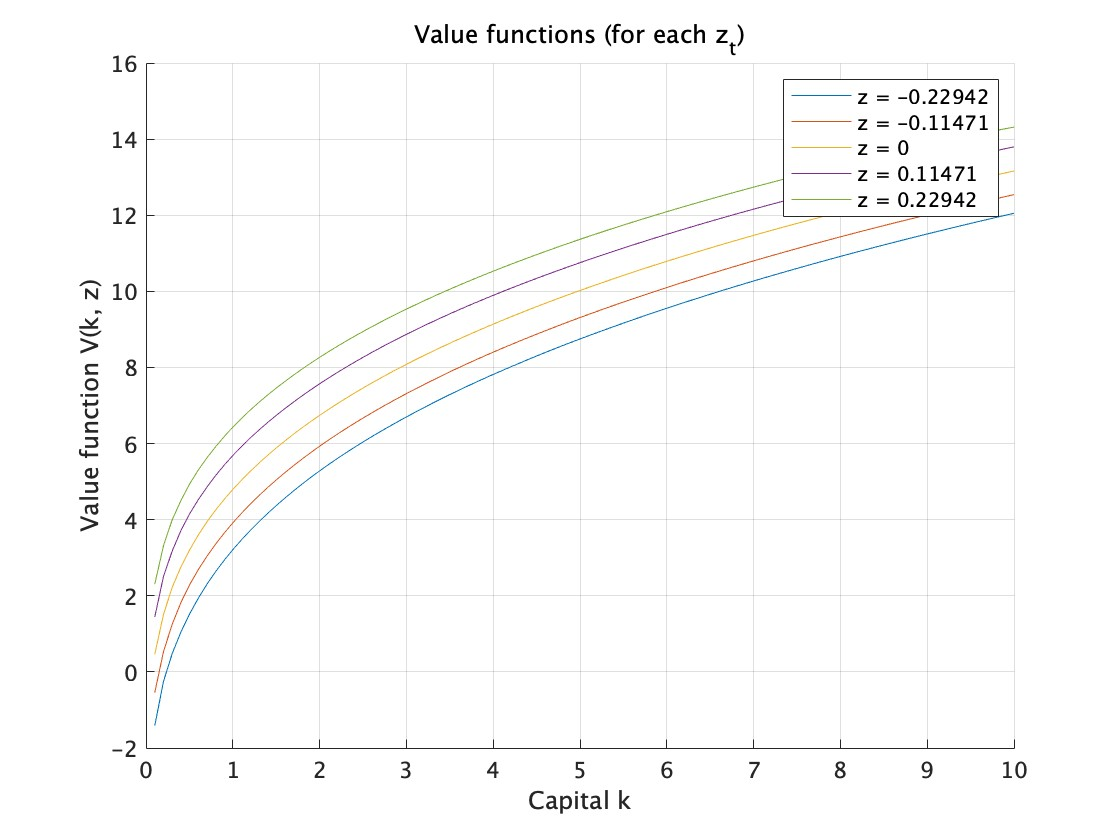
\includegraphics[width=\textwidth]{ValueFunc.jpg}
        \caption{Value function}
    \end{subfigure}
    \begin{subfigure}{0.45\textwidth}
        \centering
        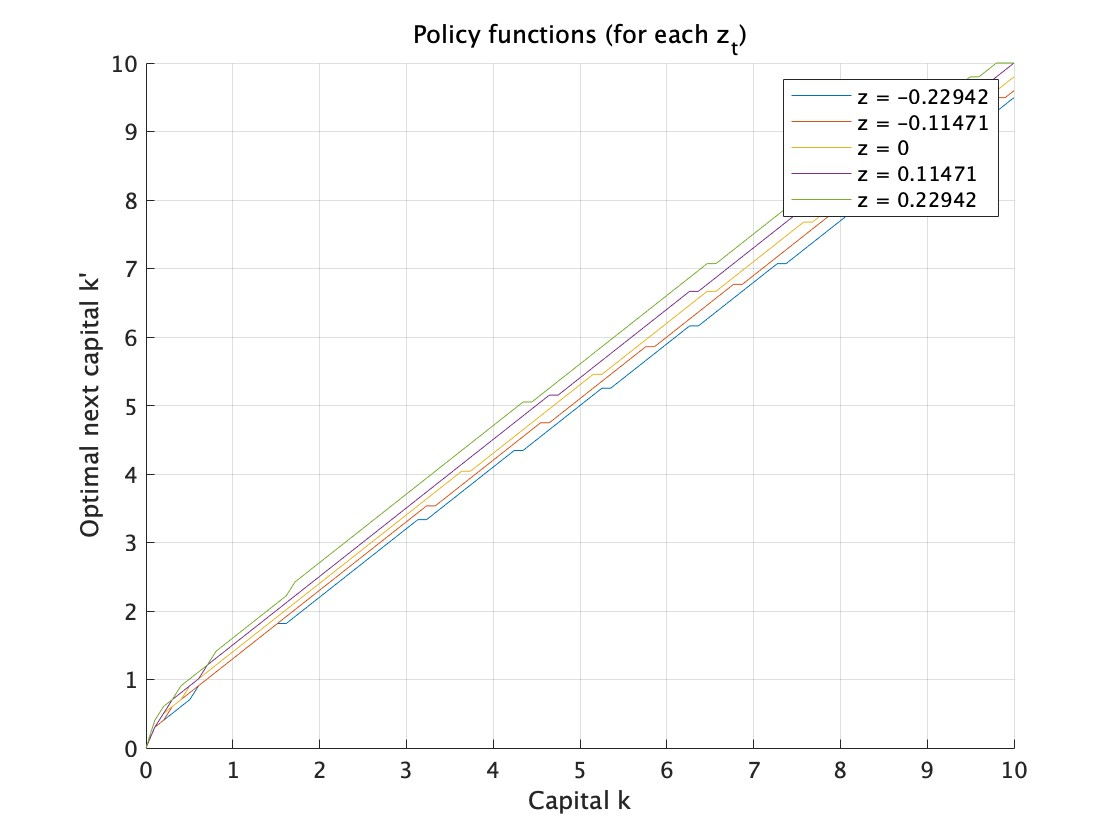
\includegraphics[width=\textwidth]{PolicyFunc.jpg}
        \caption{Policy function}
    \end{subfigure}
\end{figure}


The Matlab code is below.

\lstset{style=matlab}
\begin{lstlisting}
beta = 0.95;
alpha = 0.4;
delta = 0.06;
u = @(c) log(c);
k_min = 0;
k_max = 10;
Nk = 100;
k_grid = linspace(k_min, k_max, Nk)';

Nz = 5;
mu = 0;
rho = 0.9;
sigma = 0.1;
m = 1;
[Z,Zprob] = tauchen(Nz,mu,rho,sigma,m);

V = zeros(Nk, Nz);
policy_k = zeros(Nk, Nz);

max_iter = 1000; 
tol = 1e-6;    
for iter = 1:max_iter
    V_new = zeros(Nk, Nz);
    for i = 1:Nk
        for j = 1:Nz
            z0 = Z(j); 
            k0 = k_grid(i);

            c = exp(z0) * k0^alpha + (1 - delta) * k0 - k_grid;
            U = u(c);
            U(c <= 0) = -inf; 

            EV = V * Zprob(j,:)'; 

            total_value = U + beta * EV;

            [V_new(i,j), policy_index] = max(total_value);
            policy_k(i,j) = k_grid(policy_index);
        end
    end
    
    if max(abs(V_new(:) - V(:))) < tol
        disp(['Converged (number of iterations: ', num2str(iter), ')']);
        break;
    end
    V = V_new;
end

figure;
hold on;
for i_z = 1:Nz
    plot(k_grid, V(:, i_z), 'DisplayName', ['z = ', num2str(Z(i_z))]);
end
xlabel('Capital k');
ylabel('Value function V(k, z)');
title('Value functions (for each z_t)');
legend show;
grid on;

figure;
hold on;
for i_z = 1:Nz
    plot(k_grid, policy_k(:, i_z), 'DisplayName', ['z = ', num2str(Z(i_z))]);
end
xlabel('Capital k');
ylabel('Optimal next capital k''');
title('Policy functions (for each z_t)');
legend show;
grid on;
\end{lstlisting}

\section*{Q3}
\subsection*{(a)}
\begin{align*}
P^2 = 
    \begin{bmatrix}
    0.83 & 0.15 & 0.01 & 0.01 \\
    0.31 & 0.41 & 0.15 & 0.13 \\
    0.05 & 0.27 & 0.53 & 0.15 \\
    0.17 & 0.17 & 0.27 & 0.39
    \end{bmatrix}.
\end{align*}
For all $i,j\in \qty{1,2,3,4,}$, $P^2_{ij}>0$. Therefore, by the LS theorem 2.2.2, P has a unique stationary distribution and the process is
asymptotically stationary.



\subsection*{(b)}
Stationary distribution $\pi = (\pi_1,\pi_2,\pi_3,\pi_4)$ of $P$ satisfies
\begin{align*}
    \pi^T &= \pi^T P\\
    \begin{bmatrix}\pi_1\\\pi_2\\\pi_3\\\pi_4\end{bmatrix}
        &=\begin{bmatrix}
            0.9\pi_1 + 0.2\pi_2 + 0.0\pi_3 + 0.1\pi_4 \\
            0.1\pi_1 + 0.6\pi_2 + 0.2\pi_3 + 0.1\pi_4 \\
            0.0\pi_1 + 0.1\pi_2 + 0.7\pi_3 + 0.2\pi_4 \\
            0.0\pi_1 + 0.1\pi_2 + 0.1\pi_3 + 0.6\pi_4
            \end{bmatrix}
\end{align*}

Solving this, we have 
\begin{align*}
    \pi = (\frac{6}{11},  \frac{5}{22},  \frac{3}{22}, \frac{1}{11})
\end{align*}


\subsection*{(c)}
\subsubsection*{(i)}

\begin{align*}
    Pr(e^1_{t+1}|e^1_{t})=0.9\\
    Pr(e^1_{t+1}|e^2_{t})=0.2\\
    Pr(e^1_{t+1}|e^3_{t})=0.0\\
    Pr(e^1_{t+1}|e^4_{t})=0.1\\
    Pr(e^2_{t+1}|e^1_{t})=0.1\\
    Pr(e^3_{t+1}|e^2_{t})=0.1\\
    Pr(e^4_{t+1}|e^3_{t})=0.1
\end{align*}

Then, the likelihood is 
\begin{align*}
    \qty(\frac{6}{11}*0.9+\frac{5}{22}*0.2+\frac{3}{22}*0+\frac{1}{11}*0.1)*0.1^3=\frac{6}{11000}
\end{align*}

\subsubsection*{(ii)}

\begin{align*}
    Pr(e^1_{t+1}|e^1_{t})=0.9\\
    Pr(e^1_{t+1}|e^2_{t})=0.2\\
    Pr(e^1_{t+1}|e^3_{t})=0.0\\
    Pr(e^1_{t+1}|e^4_{t})=0.1
\end{align*}


Then, the likelihood is 
\begin{align*}
    \qty(\frac{6}{11}*0.9+\frac{5}{22}*0.2+\frac{3}{22}*0+\frac{1}{11}*0.1)*0.9^3=\frac{4374}{11000}
\end{align*}



\subsection*{(d)}

\begin{align*}
    E[y_1|e_0=e^1] = 0.9*0 + 0.1*1 = 0.1
\end{align*}


\begin{align*}
    P^5 = \begin{bmatrix}
        0.70524 & 0.19908 & 0.05284 & 0.04284 \\
        0.44100 & 0.25652 & 0.17908 & 0.12340 \\
        0.23420 & 0.27964 & 0.31708 & 0.16908 \\
        0.31476 & 0.24476 & 0.25964 & 0.18084
        \end{bmatrix}.
\end{align*}

\begin{align*}
    E[y_5|e_0=e^1] = 0.70524*0 + 0.19908*1 + 0.05284*2 + 0.04284*4 = 0.47612.
\end{align*}

\section*{Q4}

\subsection*{(a)}
A competitive Arrow-Debreu equilibrium is prices $\{\hat{p_t}(s^t)\}_{t=0, s^t \in S^t}^\infty$ and allocations $\{\hat{c_t^i}(s^t)\}_{t=0, s^t \in S^t}^\infty$ for $i = 1, 2$ such that
\begin{align*}
    \max_{\{c_t^i(s^t)\}_{t=0, s^t \in S^t}^\infty} \Sigma_{t=0}^\infty \Sigma_{s^t \in S^t} \beta^t \pi(s^t) \log c^i_t(s^t)\\
    & \text{s.t. }\Sigma_{t=0}^\infty \Sigma_{s^t \in S^t} \hat{p_t}(s^t) c^i_t(s^t) \leq \Sigma_{t=0}^\infty \Sigma_{s^t \in S^t} \hat{p_t}(s^t) e^i_t(s^t)\\
    & c^i_t \geq 0 \text{ for all }t,\text{ all }s^t \in S^t
\end{align*}
and goods market clear, i.e.,
\begin{align*}
    \hat{c^1_t}(s^t) + \hat{c^2_t}(s^t) = e^1_t(s^t) + e^2_t(s^t) \text{ for all } t, \text{ all } s^t \in S^t
\end{align*}

\subsection*{(b)}
Let $\mu^i$ be the Lagrange multiplier on the budget constraint.\\
The FOCs w.r.t. $c^i_t(s^t)$ and $c_o^i(s^0)$ are as below.
\begin{align*}
    \frac{\beta^t \pi(s^t)}{c^i_t(s^t)} = \mu^i p_t(s^t)\\
    \frac{\pi(s^0)}{c_0^i(s^0)} = \mu^i p_o(s^0)
\end{align*}
From these equations,
\begin{align*}
    \frac{p_t(s^t)}{p_0(s^0)} = \beta^t \frac{\pi(s^t)}{\pi(s^0)} \frac{c_0^i(s^0)}{c_t^i(s^t)}
\end{align*}
Thus,
\begin{align*}
    \frac{c_0^2(s^0)}{c_0^1(s^0)} = \frac{c_t^2(s^t)}{c_t^1(s^t)}
\end{align*}
holds.
Then, there exist $\theta^i \geq 0$ with $\Sigma_i \theta^i = 1$ such that
\begin{align*}
    c_t^i(s^t) = \theta^i e_t(s^t)\\
    \text{where }\theta^i = \frac{\Sigma_{t=0}^\infty \Sigma_{s^t \in S^t} p^t(s^t) e_t^i (s^t)}{\Sigma_{t=0}^\infty \Sigma_{s^t \in S^t} p^t(s^t) e_t (s^t)}\\
    \text{s.t. }\theta^1 + \theta^2 = 1
\end{align*}
with $e_t(s^t) = \Sigma_i e_t^i (s^t)$.
By using this and normalizing $p_0(s^0) = 1$,
\begin{align*}
    p_t(s^t) = \beta^t \frac{\pi(s^t)}{\pi(s^0)}\frac{e_0(s^0)}{e_t(s^t)}
\end{align*}

\subsection*{(c)}
Let $q_t(s^t, s_{t+1})$ denote price at period t of a contract that pays one unit of consumption in period $t+1$ if $t+1$ event is $s_{t+1}$.\\
Let $a_{t+1}^i(s^t, s_{t+1})$ be the quantities of Arrow securities bought at period t by agent i.\\
A sequential market equilibrium is allocations $(\hat{c^i}, \hat{a^i})_{i = 1, 2}$ and prices $\hat{q}$ such that
\begin{align*}
    & \text{For }i = 1, 2, \text{ given }\hat{q}, (\hat{c^i}, \hat{a^i})_{i = 1, 2} \text{ solves}\\
    & \max_{c^i, a^i} \log c^i_t(s^t)\\
    & \text{s.t. }\log c_t^i(s^t) + \Sigma_{s_{t+1} \in S} \hat{q_t}(s^t, s_{t+1}) \leq e_t^i(s^t) + a_t^i(s^t)\\
    & c_t^i(s^t) \geq 0\\
    & a_{t+1}^i(s^t, s_{t+1}) \geq - \bar{A^i}\\
    & \text{for all }t, s^t \in S^t \text{ and }s_{t+1} \in S.
\end{align*}
and goods markets clear, i.e.,
\begin{align*}
    & \text{For all }t \geq 0,\\
    & \Sigma_{i = 1, 2} \hat{c_t^i}(s^t) = \Sigma_{i = 1, 2} e_t^i(s^t) \text{ for all }t, s^t \in S^t\\
    & \Sigma_{i = 1, 2} \hat{a}_{t+1}^i (s^t, s_{t+1}) = 0 \text{ for all }t, s^t \in S^t \text{ and }s_{t+1} \in S
\end{align*}
In addition, the natural borrowing limit for each consumer in each state is
\begin{align*}
    \bar{A^i} = \Sigma_{t=0}^\infty \Sigma_{s^t \in S^t} p_t(s^t) e_t^i(s^t)
\end{align*}

\subsection*{(d)}
Let $q_t(s^t, s_{t+1})$ denote the price of the price of one-period state-contingent bonds.\\
From (b),
\begin{align*}
    p_t(s^t) = \beta^t \frac{\pi(s^t)}{\pi(s^0)} \frac{e_0(s^0)}{e_t(s^t)}
\end{align*}
Then,
\begin{align*}
    q_t(s^t, s_{t+1}) &= \frac{p_{t+1}(s^{t+1})}{p_t(s^t)}\\
    &= \beta \frac{\pi(s^{t+1})}{\pi(s^t)} \frac{e_t(s^t)}{e_{t+1}(s^{t+1})}
\end{align*}
For this economy, 4 price patterns exist.
\begin{enumerate}[label=(\roman*)]
    \item $q_t(s^1, s^2) = \beta \times 0.7 \times \frac{1}{3} \fallingdotseq 0.222$
    \item $q_t(s^1, s^1) = \beta \times 0.3 = 0.285$
    \item $q_t(s^2, s^1) = \beta \times 0.1 \times 3 = 0.285$
    \item $q_t(s^2, s^2) = \beta \times 0.9 = 0.855$
\end{enumerate}
Let $R_{t+1}(s^{t+1})$ be the gross return.\\
The gross returns from each bond purchased at time t are
\begin{enumerate}[label=(\roman*)]
    \item $q_t(s^1, s^1) = \beta \times 0.3 = 0.285$\\
    $R_{t+1}(s^1) = 1/0.285 \fallingdotseq 3.509$
    \item $q_t(s^2, s^1) = \beta \times 0.1 \times 3 = 0.285$\\
    $R_{t+1}(s^1) = 1/0.285 \fallingdotseq 3.509$
\end{enumerate}

\subsection*{(e)}
Let $P_t^B(d; s^t)$ denote the price of one-period risk-free bond.
\begin{align*}
    P_t^B(d; s^t) &= \frac{\Sigma_{s^{t+1}} p_{t+1}(s^{t+1})}{p_t(s^t)}\\
    &= \Sigma_{s^{t+1}} q_t(s^t, s_{t+1})
\end{align*}
Therefore, the fross return of the bond $R_{t+1}^B (s^{t+1})$ is
\begin{enumerate}[label=(\roman*)]
    \item $s^t = s^1$\\
    $P_t^B(d; s^1) = 0.285 + 0.222 = 0.507$\\
    $\therefore R_{t+1}(s^{t+1}) = 1.972$
    \item $s^t = s^2$\\
    $P_t^B(d; s^2) = 0.285 + 0.855 = 1.14$\\
    $\therefore R_{t+1}(s^{t+1}) = 0.877$
\end{enumerate}



\end{document}